\documentclass[conference]{IEEEtran}

\usepackage{graphicx,url}
\usepackage{float}
\usepackage{tikz}
\usetikzlibrary{shapes, arrows, shapes.geometric}
\usepackage{verbatim}
\usepackage[brazilian]{babel}
\usepackage[utf8]{inputenc}
\usepackage[T1]{fontenc}

\graphicspath{ {../images/} }

% correct bad hyphenation here
\hyphenation{op-tical net-works semi-conduc-tor}


\begin{document}
\title{VRSnake: um Jogo de Realidade Virtual em GPGPU}


% author names and affiliations
% use a multiple column layout for up to three different
% affiliations
% \author{\IEEEauthorblockN{BLIND REVIEW\IEEEauthorrefmark{1}}}
% \author{Adriano M. Gil\inst{1}, Thiago S. Figueira\inst{1}}
% \address{Samsung Instituto de Desenvolvimento para a Informática da Amazônia (SIDIA)\\
%   Manaus -- AM -- Brazil
%   \email{\{adriano.gil,t.figueira\}@samsung.com}
% }
% \author{\IEEEauthorblockN{BLIND REVIEW\IEEEauthorrefmark{1}}}

%SIDIA,\\
%Manaus -- AM -- Brazil}} 
\author{\IEEEauthorblockN{Thiago S. Figueira\IEEEauthorrefmark{1},
Adriano M. Gil\IEEEauthorrefmark{1}}
\IEEEauthorblockA{\IEEEauthorrefmark{1}Samsung Instituto de Desenvolvimento para a Informática da Amazônia\\
SIDIA,\\
Manaus -- AM -- Brazil}} 


\maketitle

% As a general rule, do not put math, special symbols or citations
% in the abstract
\begin{abstract}
Aplicações de realidade virtual são caracterizadas pela alta sensibilidade à atrasos na sincronização entre os movimentos do usuário e a respectiva renderização do mundo virtual. Uma forma de acelerar a execução da camada lógica de uma aplicação é transportar sua implementação para GPU. Esta última, portanto, torna-se responsável por renderizar os elementos visuais, mas também avaliar os estados da aplicação, assumindo um papel de propósito geral ou GPGPU (\textit{General Purpose Graphics Processing Unit}). Como exemplo dessa abordagem, implementamos uma versão do clássico jogo Snake em realidade virtual onde todos os elementos visuais bem como a lógica de jogo são computados via \textit{shader} em um único \textit{mesh}.
\end{abstract}
% no keywords


% For peerreview papers, this IEEEtran command inserts a page break and
% creates the second title. It will be ignored for other modes.
\IEEEpeerreviewmaketitle

% Reescrito
\section{Introdução} \label{sec:introduction}

% Unity e Pipeline Gráfica
\begin{comment}
O motor e editor gráfico \textit{Unity} é uma ferramenta comum para o desenvolvimento de software em realidade virtual e aumentada. Usualmente, uma aplicação \textit{unity} é constituída por cenas providas de um sistema lógico próprio que, uma vez agrupadas, formam todos os elementos pertinentes ao universo do jogo. Neste aspecto, a \textit{pipeline} gráfica rotineiramente utilizada pelas apliações e jogos \textit{unity} contempla, em linhas gerais, os seguintes passos:  a CPU (\textit{central processing unit}) transmite informações sobre os elementos gráficos à GPU (\textit{graphics processing unit}) através do estágio de aplicação, onde os \textit{assets} gráficos como modelos 3D e suas texturas são carregados na VRAM (\textit{video random access memory}), posteriormente durante o estágio de geometria, os objetos que devem ser renderizados bem como seus respectivos posicionamentos e demais informes visuais relevantes são tratados pela GPU e, em última instância, convertidos em imagem no estágio de rasterização \cite{akenine2008real}.
\end{comment}

A unidade gráfica de processamento (GPU, em inglês) possui unidades de processamento paralelas \cite{DBLP:journals/corr/abs-1202-4347} que podem ser usadas para diferentes finalidades além da renderização, por exemplo, para cálculos de física em jogos ou para algoritmos de aprendizagem de máquina. Desta forma, este poder computacional pode ser aproveitado em outras atividades, extendendo sua função básica de computação de imagens em jogos, por exemplo, para a manipulação de toda a lógica do jogo. 

% Proposta
Este trabalho propõe o desenvolvimento de um jogo de realidade virtual para a plataforma Gear VR através de uma arquitetura onde ambas lógica de funcionamento e renderização gráfica sejam fundamentadas em código de GPU, o \textit{shader}. Em alusão à um clássico, o jogo \textit{snake} será recriado para os dispositivos de realidade virtual Samsung em uma aplicação \textit{Unity3D}, diferencia-se do original na medida que o jogador controla, através do \textit{joystick}, o posicionamento do objeto coletável ao invés da serpente.

% Estrutura do artigo
Analisamos na seção \ref{sec:relatedworks} trabalhos correlatos. Um esclarecimento sobre as regras do jogo desenvolvido pode ser encontrado na seção \ref{sec:vrsnake}. A arquitetura proposta é detalhada na seção \ref{sec:architecture}. Apresenta-se como um jogo de realidade virtual pode ser renderizado em uma esfera invertida na seção \ref{sec:invertedsphere}. Resultados são discutidos na seção \ref{sec:results}. Por fim, pautam-se as conclusões e perspectivas de trabalhos futuros na seção \ref{sec:conclusion}.

% Reescreve explorando o GPUWars e estabelecer diferença entre este trabalho e o outro
\section{Trabalhos Relacionados} \label{sec:relatedworks}

GPUWars \cite{GPGPUWars} é um jogo bidimensional de tiro com visão \textit{top-down} (de cima para baixo) que utiliza a GPU como responsável pelo processamento da inteligência artificial, física dos corpos e por determinar o estado do jogo. O jogo \textit{Jelly in the Sky}, disponibilizado como produto na plataforma de jogos digitais \textit{Steam}, é uma simulação fisicamente realista bidimensional em GPU.

Alguns outros trabalhos, tal como visto em \cite{Joselli:2010:AGL:1658866.1658869}, fazem uso da GPU como processador auxiliar em cálculos matemáticos e físicos. Contudo, aplicações em realidade virtual, tal qual a deste artigo, diferem destas demais aplicações devido à necessidade de preencher o espaço tridimensional de forma a fornecer conteúdo para os 3 graus de liberdade (3DoF - \textit{3 Degrees of Freedom}) possibilitados pelo Gear VR.

% Reescrito
\section{VRSnake: Design do Jogo} \label{sec:vrsnake}
O \textit{VRSnake} é a versão em realidade virtual do clássico jogo 2D \textit{Snake}. No jogo original controlava-se a serpente na busca pelos coletáveis distribuídos pelo cenário, o \textit{VRSnake} permite ao jogador controlar o posicionamento destes objetos coletáveis, desta forma seu principal objetivo é derrotar as diversas serpentes, determinadas proceduralmente, que estão espalhadas no universo virtual. As regras são essencialmente as mesmas, mas o jogador vence quando resta unicamente uma serpente.

\begin{comment} Propomos então as regras como seguem:

As serpentes buscam ininterruptamente o objeto coletável posicionado pelo jogador e seguem até o objeto pelo percurso que as manterão vivas por mais tempo, isto é, as serpentes desviam de si mesmas e das demais serpentes quando possível. Se este desvio não acontece, uma das serpentes é eliminada. Em outro aspecto, caso o objeto coletável seja capturado com sucesso, a \textit{snake} cresce em uma unidade de medida. O jogador vence a partida quando resta unicamente uma serpente.
\end{comment}

%Reescrevendo
\section{Arquitetura de um Jogo GPGPU} \label{sec:architecture}
% Jogos são aplicações interativas que executam três classes de ações: coleta, processamento e exibição de dados. 
% A coleta de dados foca em recolher dados dos dispositivos de entrada sejam eles teclado, mouse, toque ou \textit{joysticks}. O processamento abrange o reconhecimento dos dados coletados e sua devida tradução para o mundo do jogo, mas também garante o cumprimento das regras e gerenciamento do estado geral da aplicação. A exibição é o passo final, pois retorna ao jogador as consequências de seus atos de maneira sensorial. 
O \textit{VRSnake} é um jogo de realidade virtual que concentra as ações das classes de processamento e exibição na unidade gráfica de processamento (GPU - \textit{Graphics Processing Unit}) através de uma textura, ao passo que a unidade central de processamento (CPU - \textit{Central Processing Unit}) é encarregada da entrada de dados. Esta arquitetura foi desenvolvida utilizando o motor gráfico \textit{Unity3D} e implementada através do HLSL (\textit{High Level Shading Language}) para os \textit{shaders} e CSharp como linguagem de programação de CPU (\textit{Central Processing Unit}).

Uma textura é utilizada para representar os estados de jogo e armazenar o posicionamento das serpentes e do objeto coletável, isto permite manipular as coordenadas do espaço 3D ao redor da câmera usando apenas coordenadas UV. A textura então serve como entrada para o \textit{shader} processar, em GPU, a correta movimentação das serpentes e renderizar os elementos de jogo em um único \textit{mesh}.

O deslocamento das serpentes até seu objetivo é realizado através de uma função utilitária de avaliação de estados que analisa cada possibilidade de movimentação dadas sua direção e orientação. Em essência, a serpente sempre está buscando alcançar o coletável, por isso avalia o curso de menor distância no eixos X e Y de UV e desde que não exista impedimentos, assume este caminho e repete o processo, conforme ilustra a equação \ref{eq_fardo}.

\begin{equation}
F(A) = R * (D + O)
\label{eq_fardo}
\end{equation}

Onde R é um fator de randomização; D representa a distância de \textit{Manhattan} entre a posição atual e o objeto coletável; e O é um valor atribuído à existência ou não de obstáculos neste trajeto.

\begin{comment}
A GPU processa e renderiza as informações de jogo, como o posicionamento das serpentes e objeto coletável, em um único \textit{mesh} ou textura, logo é possível usar o mapeamento UV desta textura para rastrear a colocação destes objetos em cena.  Isto facilita, por exemplo, a movimentação circular da serpente, pois é possível verificar as extremidades da superfície mapeada em coordenadas UV para saber se a serpente deve ser redesenhada.
\end{comment}

\section{Realidade Virtual} \label{sec:invertedsphere}
Tendo em vista que a proposta deste artigo contempla um jogo essencialmente 2D, tal como o \textit{Snake} original, tem-se o desafio de exibir informação bidimensional em um cenário 3D de forma que tudo aconteça ao redor do usuário. Para tanto, recorreu-se à projeção cilíndrica equidistante. A solução padrão adotada na exibição de imagens equiretangulares em 360 graus é a esfera invertida, ou seja, uma esfera que tenha apenas seu lado interno renderizado, pois possibilita preencher completamente todo o campo de visão do usuário. A geração procedural de uma esfera pode seguir uma das duas abordagens abaixo:
\begin{enumerate}
  \begin{item} uma icosfera, i.e. uma esfera cujos vértices são distribuídos uniformemente; \end{item}
  \begin{item} geração de vertíces baseada em coordenadas de longitude/latitude. \end{item}
\end{enumerate}

% TODO: Refrasear texto
Para este trabalho, preferiu-se a segunda abordagem devido ao mapeamento de UV adotado ser o padrão para \textit{softwares} de modelagem na geração de esferas: vértices gerados a partir de coordenadas de longitude/latitude. Neste aspecto, as equações abaixo ilustram este processo:

% 2 - Mapeamento de UV em uma esfera invertida

A posição Y dos pontos da esfera, considerando raio unitário, pode ser dada pela equação \ref{equation2}.
\begin{equation}
y_{i} = \cos(\alpha_{yi})
\label{equation2}
\end{equation}

Obtém-se as posições X e Z dos vértices da esfera em função de suas coordenadas de longitude e latitude através das equações \ref{equation3} e \ref{equation4}.

\begin{equation}
x_{i} = \sin(\alpha_{yi}) * \sin(\alpha_i)
\label{equation3}
\end{equation}

\begin{equation}
z_{i} = \sin(\alpha_{yi}) * \cos(\alpha_i)
\label{equation4}
\end{equation}

\section{Resultados} \label{sec:results}
Desenvolveu-se em realidade virtual o jogo \textit{Snake} no ambiente de desenvolvimento \textit{Unity3D}. Gerou-se uma aplicação \textit{Android} testada no \textit{Samsung Galaxy S8} através do \textit{Gear VR} com o controle de modelo ET-YO32. A imagem abaixo ilustra a taxa de quadros, métrica utilizada em \cite{GPGPUWars} e \cite{GPGPUTechniques}, no \textit{GearVR} através da ferramenta de avaliação de performance da \textit{Oculus}, o \textit{OVR Metrics Tool}:

\begin{figure}[H] 
\centering
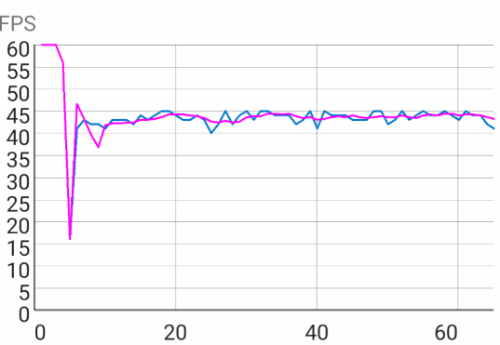
\includegraphics[scale=0.5]{VRPerformance}
\caption{Quadros-por-segundo conforme o OVR Metrics Tool executado durante a execução da aplicação} \label{fig:VRPerformance}
\end{figure}

A aplicação apresentou taxa média de 43.96 \textit{fps} (\textit{frames-per-second}, quadros-por-segundo), com mínima de 16 \textit{fps} e máxima de 60 \textit{fps}. Conforme visto na figura \ref{fig:VRPerformance}, a aplicação não mantém estavéis 60 \textit{fps} recomendados pela \textit{Oculus} \cite{OculusVRGuidelines}, acreditamos que isto se deve aos processos de comunicação entre CPU-GPU, mas também à possíbilidade de melhorias nos códigos escritos em \textit{shader}.

\section{Conclusão}\label{sec:conclusion}
% Resumo do artigo
Apresentamos a implementação de um jogo em realidade virtual que distribui passos usualmente restritos à CPU, tais como lógica de jogo e movimentação, para a GPGPU, através de \textit{shaders}. Houveram outras abordagens que adotaram o mesmo desafio, no entanto, foram restritas ao universo bidimensional. Mostramos, portanto, a viabilidade desta arquitetura para jogos de realidade virtual ainda que para a renderização auxiliar a fim de aliviar os encargos da CPU. 

% Trabalhos Futuros
Para trabalhos futuros, há dois grandes marcos em vista: permitir uma experiência mais agradável e estável através dos 60 \textit{fps} e otimizar os processos de comunicação CPU-GPU.

\bibliographystyle{IEEEtran}

\bibliography{bare_conf}
\end{document}


